\section*{Aufgabe 3 (30 Punkte)}
\vspace{0.4cm}
\subsection*{\frage{1}{4}}
Der  Grenzwert
\begin{align*}
\lim \limits_{x\to 0} 
\frac{e^x + e^{-x} -2}{1 - \cos(x)}
\end{align*}
ist
\renewcommand{\labelenumi}{(\alph{enumi})}
\begin{enumerate}
	\item 
	$ 0 $.
	\item
	$ 0.5 $.
	\item
	$ 1 $.
	\item
	$ 2 $.
\end{enumerate}
\ \\
\textbf{Lösung:}
\begin{mdframed}
\underline{\textbf{Vorgehensweise:}}
\renewcommand{\labelenumi}{\theenumi.}
\begin{enumerate}
\item Wende die Regel von de l'H\^{o}pital an.
\end{enumerate}
\end{mdframed}

\underline{1. Wende die Regel von de l'H\^{o}pital an}\\

Durch zweimaliges Anwenden der Regel von de l'H\^{o}pital erhalten wir:
\begin{align*}
\lim \limits_{x \to 0}
\frac{e^x + e^{-x} -2}{1 - \cos(x)}
=
\lim \limits_{x \to 0}
\frac{e^x - e^{-x}}{ \sin(x)}
=
\lim \limits_{x \to 0}
\frac{e^x + e^{-x}}{ \cos(x)}
=
\frac{e^0 + e^{0}}{ \cos(0)} = \frac{1+1}{1} = 2. 
\end{align*}
\ \\
Damit ist Antwort (d) korrekt.
 
\newpage

\subsection*{\frage{2}{4}}
Der Grenzwert
\begin{align*}
\lim \limits_{x \to 3} 
\left(\frac{1}{x-3} - \frac{27}{x^3 - 27}\right)
\end{align*}
ist
\renewcommand{\labelenumi}{(\alph{enumi})}
\begin{enumerate}
	\item 
	$ 0 $.
	\item
	$ \frac{1}{3} $.
	\item
	$ \frac{2}{5} $.
	\item
	$ \infty $.
\end{enumerate}
\ \\
\textbf{Lösung:}
\begin{mdframed}
\underline{\textbf{Vorgehensweise:}}
\renewcommand{\labelenumi}{\theenumi.}
\begin{enumerate}
\item Überlege dir einen Zusammenhang für die Nenner der Brüche.
\item Berechne den Grenzwert. 
\end{enumerate}
\end{mdframed}

\underline{1. Überlege dir einen Zusammenhang für die Nenner der Brüche}\\
Wegen
\begin{align*}
x^3 - 27 = 0 \ \Leftrightarrow  \
x^3 = 27 \ \Leftrightarrow \
x = \sqrt[3]{27} = 3
\end{align*}
ist $ 3  $ eine Nullstelle von $ x^3 - 27 $. Durch Polynomdivision erhalten wir dann:
\begin{align*}
(x^3 - 27) : (x-3) = x^2 + 3x + 9
\ \Leftrightarrow \
x^3 - 27 = ( x-3)(x^2 +3x +9).
\end{align*}
Demnach erhalten wir 
\begin{align*}
\frac{1}{x-3} - \frac{27}{x^3 -27}
&=
\frac{1}{x-3} - \frac{27}{( x-3)(x^2 +3x +9)}
=
\frac{x^2 +3x +9}{( x-3)(x^2 +3x +9)} - \frac{27}{( x-3)(x^2 +3x +9)}\\
&=
\frac{x^2 +3x -18}{( x-3)(x^2 +3x +9)}
=
\frac{(x-3)(x+6)}{( x-3)(x^2 +3x +9)}
=
\frac{x+6}{x^2 +3x +9}.
\end{align*}
\\

\underline{2. Berechne den Grenzwert}\\
Mit unseren Vorüberlegungen gilt
\begin{align*}
\lim \limits_{x \to 3} 
\left(\frac{1}{x-3} - \frac{27}{x^3 - 27}\right)
=
\lim \limits_{x \to 3} 
\frac{x+6}{x^2 +3x +9}
=
\frac{9}{27} = \frac{1}{3}
\end{align*}
\ \\
Also ist Antwort (b) korrekt.
\newpage
\subsection*{\frage{3}{4}}
Am $ 26.12.2017 $ entdeckte der Hobby-Mathematiker Jonathan Price aus Germantown, Tennessee, die bislang grösste bekannte Primzahl $ p $, nämlich
\begin{align*}
p = 2^{77'232'917} -1
\end{align*}
Wie viele Stellen hat $ p $ im Dezimalsystem?\\
(\textit{Tipp:} Überlegen Sie sich den Zusammenhang zwischen Anzahl Stellen einer natürlichen Zahl $ n $ im Dezimalsystem und ihrem Zehnerlogarithmus $ \log_{10}(n) $) 
\renewcommand{\labelenumi}{(\alph{enumi})}
\begin{enumerate}
	\item 
	$ p $ hat im Dezimalsystem $ 23'249'424 $ Stellen.
	\item
	$ p $ hat im Dezimalsystem $ 23'249'425 $ Stellen.
	\item
	$ p $ hat im Dezimalsystem $ 53'533'778 $ Stellen.
	\item
	$ p $ hat im Dezimalsystem $ 53'533'779 $ Stellen.
\end{enumerate}
\ \\
\textbf{Lösung:}
\begin{mdframed}
\underline{\textbf{Vorgehensweise:}}
\renewcommand{\labelenumi}{\theenumi.}
\begin{enumerate}
\item Welchen Zusammenhang gibt es zwischen natürlichen Zahlen und Zehnerpotenzen.
\item  Wende diesen Zusammenhang an.
\end{enumerate}
\end{mdframed}

\underline{1. Welchen Zusammenhang gibt es zwischen natürlichen Zahlen und Zehnerpotenzen}\\
Sei $ n \in \mathbb{N} $ eine natürliche Zahl mit $ s $ Stellen.
Dann lässt sich diese durch 
\begin{align*}
n = x 10^{s-1}
\end{align*}
mit $ x \in [1,10) $ darstellen.
Damit gilt
\begin{align*}
\log_{10} (n) = \log_{10} (x) + (s-1) 
\ \Leftrightarrow \
s = \log_{10}(n) - \log_{10}(x) + 1.
\end{align*}
Wegen $ \log_{10}(x) \in [0,1) $ folgt 
\begin{align*}
s \leq \log_{10}(n) +1.
\end{align*}
\ \\
\underline{2. Wende diesen Zusammenhang an}\\
Für eine große Zahl $ x $ ist die Differenz 
von $ \log_{10}(x) $ und $ \log_{10}(x+1) $ sehr klein.\\
\textit{Hinweis:} Überlege dir, wie du dies mit der Ableitung von $ \log_{10}(x)  $ begründen kannst.\\
Nun gilt 
\begin{align*}
\log_{10}(p) +1 
&\approx
\log_{10}(p+1) +1\\
&=
\log_{10}(2^{77'232'917}) +1\\
&=
77'232'910 \frac{\ln(2)}{\ln(10)}+ 1 \\
&\approx
23'249'424.7 + 1
= 23'249'425.7.
\end{align*}
Mit unseren Vorüberlegungen hat $ p $ genau $ 23'249'425 $ Dezimalstellen.



\newpage
\subsection*{\frage{4}{3}}
Gegeben sei die Funktion in zwei reellen Variablen
\begin{align*}
f : D_f \to \mathbb{R}, (x,y) \mapsto
z = f(x,y) = \sqrt[4]{4x^2 + 4 y^2 - 36}
+ \frac{1}{\sqrt{x^2 - y -2}}.
\end{align*}
Welches der folgenden Bilder zeigt grau schraffiert den Definitionsbereich $ D_f \subset \mathbb{R}^2 $ von $ f $?
\renewcommand{\labelenumi}{(\alph{enumi})}
\begin{center}
	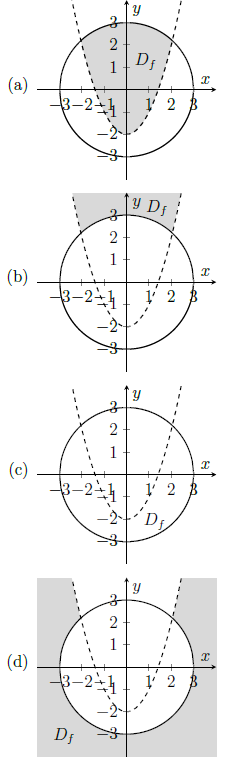
\includegraphics{pictures/auf3_4}
\end{center}
\newpage
\textbf{Lösung:}
\begin{mdframed}
\underline{\textbf{Vorgehensweise:}}
\renewcommand{\labelenumi}{\theenumi.}
\begin{enumerate}
\item Bestimme den Definitionsbereich der Funktion.
\end{enumerate}
\end{mdframed}

\underline{1. Bestimme den Definitionsbereich der Funktion}\\
Damit unsere Funktion definiert ist, müssen 
\begin{align*}
4x^2 +4y^2 - 36 &\geq 0\\
x^2 -y -2 &> 0
\end{align*}
erfüllt sein.
Zuerst kümmern wir uns um die erste Ungleichung.
Es gilt
\begin{align*}
4x^2 + 4y^2 - 36 \geq 0 \ \Leftrightarrow \
4x^2 + 4y^2 \geq 36 
\ \Leftrightarrow \
x^2 + y^2 \geq 9 = 3^2. 
\end{align*}
Diese Ungleichung beschreibt also die Fläche auf und außerhalb des Kreises mit Radius 3.
Nun zu der zweiten Ungleichung. Hierfür ist
\begin{align*}
x^2 - y - 2 > 0 
\ \Leftrightarrow \
y < x^2 -2  
\end{align*}
erfüllt. Dadurch werden alle Werte unter der um $ 2 $ nach unten verschobenen Normalparabel beschrieben.
Demnach kann nur Antwort (d) richtig sein.\\
\\
Die korrekte Antwort ist (d).
\newpage

\subsection*{\frage{5}{4}}
Betrachte die Funktion
\begin{align*}
f : D_f \to \mathbb{R}, 
(x,y) \mapsto z = f(x,y) = \ln(\sqrt{e} -x^2 -y^2)
\end{align*}
mit dem Definitionsbereich
\begin{align*}
D_f
= \{
(x,y) \in \mathbb{R}^2 : x^2 + y^2 \leq \sqrt{e}
\}.
\end{align*}
Dann ist das Bild $ R_f $ von $ f $ gegeben durch
\renewcommand{\labelenumi}{(\alph{enumi})}
\begin{enumerate}
	\item 
	$R_f = \mathbb{R} $.
	\item
	$R_f = \left( -\frac{1}{2}, \frac{1}{2} \right) $.
	\item
	$R_f = \left(  \frac{1}{2}, \infty \right) $.
	\item
	$R_f = \left( -\infty, \frac{1}{2} \right) $.
\end{enumerate}

\ \\
\textbf{Lösung:}
\begin{mdframed}
\underline{\textbf{Vorgehensweise:}}
\renewcommand{\labelenumi}{\theenumi.}
\begin{enumerate}
\item Finde die korrekte Antwort durch Äquivalenzumformungen.
\item 
Alternativer Lösungsweg.
\end{enumerate}
\end{mdframed}

\underline{1. Finde die korrekte Antwort durch Äquivalenzumformungen}\\
Wir wissen, dass $ (x,y) $ in $ D_f $ liegt genau dann, wenn
\begin{align*}
0 < \sqrt{e} - x^2 -y^2 \leq \sqrt{e} 
\end{align*}
erfüllt ist. Wegen $ \ln (x) \to -\infty $ für $ x \to 0 $ ist äquivalent zu:
\begin{align*}
- \infty < \ln (\sqrt{e} -x^2 -y^2) \leq \ln(e^{\frac{1}{2}})
\Leftrightarrow
- \infty < \ln (\sqrt{e} -x^2 -y^2) \leq \frac{1}{2}
\ \Leftrightarrow \
f(x,y) \in \left( -\infty , \frac{1}{2} \right].
\end{align*}
Damit ist Antwort (d) korrekt.\\
\\
\underline{2. Alternativer Lösungsweg}\\
Wir wissen, dass 
\begin{align*}
\lim \limits_{t\to 0} \ln(t) = - \infty
\end{align*}
gilt. Wir setzen $ t = x^2 + y^2 $, womit wir 
\begin{align*}
\lim \limits_{t \to \sqrt{e}} \ln(\sqrt{e} - t ) = -\infty
\end{align*}
erhalten. Wegen $ 0 \leq t < \sqrt{e}  $ folgt aufgrund von
\begin{align*}
\ln(\sqrt{e}) = \ln(e^{\frac{1}{2}}) = \frac{1}{2} \ln(e) = \frac{1}{2},
\end{align*}
dass $ f(x,y) \in \left( - \infty , \frac{1}{2} \right] $ gilt.\\
\\
Somit ist Antwort (d) korrekt.
\newpage

\subsection*{\frage{6}{4}}
Betrachte die Funktion
\begin{align*}
f :D_f \to \mathbb{R},
(x,y) \mapsto
z = f(x,y) = \ln \left( \left| \frac{y+1}{x-2} \right|\right).
\end{align*}
Die Steigung $ m $ der Tangenten an die Niveaulinie $ f(x,y) = \ln(2) $ im Punkt $ (x_0,y_0) = (1,1) $ ist gegeben durch
\renewcommand{\labelenumi}{(\alph{enumi})}
\begin{enumerate}
	\item 
	$ m = -0.5 $.
	\item
	$ m = 0.5 $.
	\item
	$ m = -2 $.
	\item
	Es ist nicht möglich, die Steigung $ m $ als Funktion von $ x $ anzugeben.
\end{enumerate}
\ \\
\textbf{Lösung:}
\begin{mdframed}
\underline{\textbf{Vorgehensweise:}}
\renewcommand{\labelenumi}{\theenumi.}
\begin{enumerate}
\item Wir wenden den Satz der impliziten Funktion an.
\end{enumerate}
\end{mdframed}

\underline{1. Wir wenden den Satz der impliziten Funktion an}\\
Für jede klein genug gewählte Umgebung von $ (1,1) $ gilt $ y+ 1>0 $ und $ x-2 < 0 $.
Damit folgt $ |y+1| = y+ 1 $ und $ |x-2| = 2-x $ für $ (x,y) \in U $.
Also gilt
\begin{align*}
f(x,y) = \ln \left(\frac{y+1}{2-x}\right)
= \ln(y+1) - \ln(2-x)
\end{align*}
für alle  $ (x,y) \in U $. Weiter erhalten wir 
\begin{align*}
f_x(x,y) &= -\frac{1}{2-x} \cdot (-1)=  \frac{1}{2-x}\\
f_y(x,y) &= \frac{1}{y+1}.
\end{align*}
Der Satz von der impliziten Funktion liefert nun:
\begin{align*}
m = y^\prime(1) =
-\frac{f_x(1,1)}{f_y(1,1)} 
=
- \frac{\frac{1}{2-1}}{\frac{1}{1+1}}
= - \frac{1}{\frac{1}{2}} = -2.
\end{align*}
\ \\
Also ist Antwort (c) korrekt.



\newpage



\subsection*{\frage{7}{3}}
Gegeben sind die Funktionen
\begin{align*}
f(x,y) =  \ln
\left( x^2 \sqrt{y} + \sqrt[4]{x^3 y^7}\right) - \frac{5}{2} \ln(x).
\end{align*}
wobei $ x> 0 $, $ y >0  $.
\renewcommand{\labelenumi}{(\alph{enumi})}
\begin{enumerate}
	\item
	$ f $ ist homogen vom Grad $ 0 $.
	
	\item 
	$ f $ ist linear homogen.
	\item
	$ f $ ist homogen vom Grad $ \frac{5}{2} $.
	\item
	$ f $ ist nicht homogen.
\end{enumerate}
\ \\
\textbf{Lösung:}
\begin{mdframed}
\underline{\textbf{Vorgehensweise:}}
\renewcommand{\labelenumi}{\theenumi.}
\begin{enumerate}
\item Rechne die Homogenitätseigenschaft nach.
\end{enumerate}
\end{mdframed}

\underline{1. Rechne die Homogenitätseigenschaft nach}\\
Die Funktion ist homogen vom Grad $ k $, falls 
\begin{align*}
f(\lambda x, \lambda y) = \lambda^k f(x,y)
\end{align*}
für $ \lambda > 0 $ gilt. Diese Eigenschaft werden wir nun nachrechnen:
\begin{align*}
f(\lambda x, \lambda y) &= 
\ln \left( 
(\lambda x)^2 \sqrt{\lambda y} + \sqrt[4]{(\lambda x)^3 (\lambda y)^7} 
\right)
- \frac{5}{2} \ln(\lambda x )\\
&=
\ln \left( 
\lambda^2 x^2 \lambda^{\frac{1}{2}} \sqrt{ y} +  \lambda^{\frac{10}{4}} \sqrt[4]{ x^3  y^7} 
\right)
- \frac{5}{2} \ln( x ) - \frac{5}{2} \ln(\lambda  )\\
&=
\ln \left( 
\lambda^{\frac{5}{2}} \left( x^2  \sqrt{ y} +   \sqrt[4]{ x^3  y^7} 
\right) \right)
- \frac{5}{2} \ln( x ) - \frac{5}{2} \ln(\lambda  )\\
&=
\ln\left(\lambda^{\frac{5}{2}} \right)+
\ln \left( 
 x^2 \sqrt{ y} +   \sqrt[4]{ x^3  y^7} \right) 
- \frac{5}{2} \ln( x ) - \frac{5}{2} \ln(\lambda  )\\ 
&=
\frac{5}{2}\ln\left(\lambda \right)+
\ln \left( 
x^2 \sqrt{ y} +   \sqrt[4]{ x^3  y^7} \right) 
- \frac{5}{2} \ln( x ) - \frac{5}{2} \ln(\lambda  )\\
&= \lambda^0 f(x,y)
\end{align*}
Damit ist $ f  $ homogen vom Grad $ 0 $.\\
\\
Also ist Antwort (a) korrekt.
\newpage

\subsection*{\frage{8}{4}}
Gegeben sei die Funktion
\begin{align*}
f(x,y) = 
7x\sqrt{y^a} + 3y^2 \sqrt[4]{x^a y^b} - x^2 y^{0.2},
\end{align*}
wobei $ x > 0 $, $ y > 0 $ und $ a,b \in \mathbb{R} $.\\
Für welche Werte von $ a $ und $ b $ ist $ f  $ homogen?
\renewcommand{\labelenumi}{(\alph{enumi})}
\begin{enumerate}
	\item 
	$a = 2.4$, $ b = -2 $.
	\item
	$a = 2.4$, $ b = -1.6 $.
	\item
	$a = 2$, $ b = -1.2 $.
	\item
	$ f  $ ist homogen für alle $ a,b \in \mathbb{R} $.
\end{enumerate}\
\\
\textbf{Lösung:}
\begin{mdframed}
\underline{\textbf{Vorgehensweise:}}
\renewcommand{\labelenumi}{\theenumi.}
\begin{enumerate}
\item Rechne die Homogenitätseigenschaft nach.
\item Bestimme $ a  $ und $ b $.
\end{enumerate}
\end{mdframed}

\underline{1. Rechne die Homogenitätseigenschaft nach}\\
Durch Nachrechnen erhalten wir:
\begin{align*}
f(\lambda x, \lambda y ) 
&=
7 (\lambda x) \sqrt{(\lambda y)^a}
+
3 (\lambda y)^2 \sqrt[4]{(\lambda x )^a (\lambda y )^b} - (\lambda x)^2 (\lambda y)^{0.2}\\
&=
\lambda^{1 + \frac{1}{2} a} 7x \sqrt{y^a}
+
\lambda^{2 + \frac{1}{4} a + \frac{1}{4} b}
3 y^2 \sqrt[4]{x^a y^b} - \lambda^{2.2} x^2 y^{0.2}.
\end{align*}
\ \\
\underline{2. Bestimme $ a  $ und $ b $}\\
Wir sehen, dass $ f $ nur homogen sein kann, wenn
\begin{align*}
1 + \frac{1}{2} a = 2.2 = 2 + \frac{1}{4} a + \frac{1}{4} b
\end{align*}
erfüllt ist.
Damit erhalten wir 
\begin{align*}
1 + \frac{1}{2} a = 2.2 
\ \Leftrightarrow \
\frac{1}{2} a = 1.2 
\ \Leftrightarrow \
a = 2.4
\end{align*}
und 
\begin{align*}
2 + \frac{1}{4} 2.4 + \frac{1}{4} b = 2.6 + \frac{1}{4} b = 2.2 
\ \Leftrightarrow \
b = - 1.6.
\end{align*}
\ \\ 
Also ist Antwort (b) korrekt.